\documentclass[a4paper,11pt]{article}
\usepackage[utf8]{inputenc}
\usepackage[italian]{babel}
\usepackage{amsmath, amssymb}
\usepackage{listings}
\usepackage{color}
\usepackage{xcolor}
\usepackage{times}
\usepackage{geometry}
\usepackage{graphicx}
\usepackage{listings}
\usepackage{hyperref}
\usepackage[utf8]{inputenc}

\geometry{a4paper, margin=1in}

% Colors for code listings
\definecolor{commentgray}{gray}{0.5}
\definecolor{stringgreen}{rgb}{0,0.6,0}
\definecolor{keywordblue}{rgb}{0,0,0.6}

% Listing settings for code
\lstset{
    basicstyle=\ttfamily\small,
    keywordstyle=\color{keywordblue},
    stringstyle=\color{stringgreen},
    commentstyle=\color{commentgray}\itshape,
    breaklines=true,
    frame=none,
    numbers=none,
    numberstyle=\tiny,
    tabsize=2,
    showstringspaces=false,
    captionpos=b
}

\geometry{top=3cm, bottom=3cm, left=3cm, right=3cm}


\begin{document}

% Inserisci il logo (spazio riservato)
\begin{center}
    
\includegraphics[width=3cm]{logo.png}
\end{center}

% Titolo dell'università
\begin{center}
    \textsc{\textbf{Università degli Studi di Urbino}}\\
    \textsc{Dipartimento di Scienze Pure e Applicate}\\
    \textsc{Corso di Laurea in Informatica Applicata}
\end{center}

\vspace{2cm}

% Titolo del progetto
\begin{center}
    \textbf{\Large Progetto di Programmazione Logica e Funzionale}
\end{center}

\vspace{2cm}

% Informazioni dello studente
\begin{center}
    \textbf{di Giaconi Christian, Giacomo Rossi} \\ % Spazio per il nome dello studente
    \textbf{Matricola 314045, 314671} \\ % Spazio per la matricola
    \textbf{Anno di corso: terzo}
\end{center}

\vspace{2cm}

% Anno accademico e docente
\begin{center}
    \textbf{Anno Accademico 2023/2024 - Sessione invernale}\\
    \vspace{1cm}
    \textbf{Docente: Prof. Marco Bernardo}
\end{center}

\newpage
\tableofcontents

\newpage
\section{Specifica del problema}
\textit{Scrivere un programma Haskell e un programma Prolog per implementare un sistema di raccomandazione di canzoni. Il programma legge le canzoni espresse in quattro attributi: titolo, artista, genere musicale e punteggio; da un file con valori separati da virgole, il cui nome viene acquisito da tastiera e le suggerisce all’utente basandosi sulle sue preferenze musicali, utilizzando un punteggio di gradimento acquisito da tastiera e configurato su uno o più generi, per creare una classifica con le canzoni ordinate secondo il punteggio ponderato da quello di gradimento del o dei generi musicali.}

\newpage
\section{Analisi del problema}
\subsection{Dati in ingresso}
\begin{itemize}
    \item Un file di valori separati da virgole contenenti le canzoni nel formato:
    \begin{verbatim}
    Titolo,Artista,Genere,Punteggio
    \end{verbatim}
    \item Una lista di generi preferiti.
    \item Pesi numerici assegnati ai generi preferiti.
\end{itemize}

\subsection{Dati in uscita}
\begin{itemize}
    \item Una classifica ordinata di canzoni basata sui punteggi ponderati.
    \item Una lista dei generi impostati come preferiti con il rispettivo peso associato.
\end{itemize}

\subsection{Relazioni intercorrenti}
Ogni canzone è definita da quattro attributi principali:
\begin{itemize}
    \item \textbf{Titolo}: la denominazione della canzone.  
    \item \textbf{Artista}: l’autore o il gruppo musicale che l’ha prodotta.  
    \item \textbf{Genere}: la categoria musicale di appartenenza (ad esempio, pop, rock, jazz).  
    \item \textbf{Punteggio}: una valutazione numerica che rappresenta il grado di apprezzamento della canzone.  
\end{itemize}

Il \textbf{Punteggio Ponderato} viene calcolato secondo la seguente formula:
\begin{center}
    \textit{
    \[
    \text{Punteggio Ponderato} =
    \begin{cases} 
      \text{Punteggio} \times \text{Peso Genere}, & \text{se il genere è preferito dall’utente} \\
      \text{Punteggio originale}, & \text{altrimenti}
    \end{cases}
    \]
    }
\end{center}

\noindent
Il \textbf{Peso Genere} rappresenta un coefficiente che riflette il livello di preferenza dell’utente verso un determinato genere musicale. Ciò consente di personalizzare la valutazione delle canzoni, attribuendo maggiore rilevanza ai generi di interesse senza tuttavia escludere le altre categorie, bilanciando così criteri oggettivi e preferenze soggettive.  

\newpage
\section{Progettazione dell'algoritmo}
\subsection{Scelte di progetto}
Il programma acquisisce da tastiera dati di diverso tipo, tra cui: valori \textbf{interi} per selezionare opzioni nel menu, valori \textbf{decimali} per indicare il peso attribuito ad un genere e \textbf{stringhe} per indicare il nome del file da cui si intende leggere o per indicare il/i generi che si intendono impostare come preferiti; pertanto è fondamentale una validazione stretta che si occupi di assicurare l’assenza di eccezioni dovute all’inserimento inappropriato dei dati richiesti.


\newpage
\subsection{Passi dell'algoritmo}
I passi principali dell'algoritmo, comuni sia per l'implementazione in Haskell che in Prolog, sono i seguenti:

\begin{enumerate}
    \item \textbf{Caricare le canzoni:} 
    \begin{itemize}
        \item In Haskell, le canzoni vengono caricate da un file di testo, che permette la costruzione di una lista di canzoni.
        \item In Prolog, le canzoni sono definite all’interno del programma attraverso il predicato \texttt{carica\_canzoni/0}.
    \end{itemize}
    \item \textbf{Inserire le preferenze dell'utente:} 
    L’utente fornisce i generi musicali preferiti e i relativi pesi, che influenzeranno il calcolo dei punteggi ponderati.
    \item \textbf{Calcolare i punteggi ponderati:} 
    Per ogni canzone, viene calcolato un punteggio combinando il peso associato al genere con il punteggio individuale della canzone.
    \item \textbf{Ordinare le canzoni per punteggio ponderato:} 
    Le canzoni vengono ordinate in ordine decrescente rispetto al punteggio ponderato, così da ottenere una classifica delle raccomandazioni.
    \item \textbf{Stampare la classifica:} 
    L’algoritmo produce in output la lista ordinata delle canzoni con i rispettivi punteggi, offrendo una chiara visualizzazione per l’utente.
\end{enumerate}

La ricorsività è utilizzata in entrambi i linguaggi per garantire la gestione dinamica dei dati:

\begin{itemize}
    \item \textbf{Haskell:} 
    Le funzioni ricorsive vengono impiegate per elaborare le liste di canzoni. Ad esempio, il calcolo dei punteggi ponderati viene implementato tramite una funzione che scorre ricorsivamente l’intera lista, applicando il peso corrispondente al genere di ciascuna canzone.
    \item \textbf{Prolog:} 
    L’ordinamento delle canzoni si basa su un predicato ricorsivo che inserisce ogni elemento in una lista ordinata. La dinamica di Prolog consente inoltre di aggiungere o aggiornare i generi preferiti senza ridefinire l’intera base di conoscenza.
\end{itemize}

\newpage
\section{Implementazione dell'algoritmo}
\subsection{Implementazione in Haskell}
Il file \texttt{raccomandazioni.hs} implementa l'algoritmo in Haskell. Un esempio di calcolo dei punteggi ponderati:
\begin{lstlisting}[language=Haskell]
-- #########################################################
-- # Corso di Programmazione Logica e Funzionale           #
-- # Progetto di raccomandazione di canzoni                #
-- # Studente: Giaconi Christian, Giacomo Rossi            #
-- # Matricola: 314045, 314671                             #
-- #########################################################

{-  Specifica: scrivere un programma Haskell per implementare un sistema di raccoandazione di canzoni.
    Il programma legge le canzoni espresse in quattro attributi: titolo, artista,
    genere musicale e punteggio; da un file con valori separati da virgole, il cui nome viene acquisito
    da tastiera e le suggerisce all’utente basandosi sulle sue preferenze musicali, utilizzando un
    punteggio di gradimento acquisito da tastiera e configurato su uno o più generi, per creare una
    classifica con le canzoni ordinate secondo il punteggio ponderato da quello di gradimento del
    o dei generi musicali.
-}

module Main where

-- Caricamento delle funzioni necessarie per le operazioni
import Data.List (sortOn, nub, intercalate)
import Data.Maybe (mapMaybe)
import Data.Ord (Down(..))
import qualified Data.Map as Map
import System.IO.Error(isDoesNotExistError)
import Control.Exception (catch, IOException)
import Text.Read (readMaybe)

-- #########################################################
-- Definizioni dei tipi di dati
-- #########################################################

{- La struttura 'Canzone' rappresenta una canzone con:
   - titolo: il titolo della canzone;
   - artista: l'artista che la interpreta;
   - genere: il genere musicale della canzone;
   - punteggio: un punteggio assegnato (da 1 a 10). -} 
data Canzone = Canzone
    { titolo    :: String
    , artista   :: String
    , genere    :: String
    , punteggio :: Int
    } deriving (Show, Eq)

{- PesiGeneri è una mappa che associa un genere musicale a un peso
   che influenza la priorità delle raccomandazioni. -}
type PesiGeneri = Map.Map String Double

-- #########################################################
-- Menu interattivo
-- #########################################################

{- Azione principale che avvia il menu interattivo. -}
main :: IO ()
main = menuLoop Nothing Map.empty

{- Funzione che gestisce il menu principale, mantenendo lo stato del sistema:
   - maybeCanzoni: un elenco opzionale delle canzoni caricate.
   - pesi: i pesi dei generi preferiti, gestiti dall'utente. -}
menuLoop :: Maybe [Canzone] -> PesiGeneri -> IO ()
menuLoop maybeCanzoni pesi = do
    putStrLn "\n--- Sistema di Raccomandazione Musicale ---"
    putStrLn "1. Carica un file con le canzoni"
    putStrLn "2. Gestisci i generi preferiti (aggiungi o modifica)"
    putStrLn "3. Stampa la classifica delle canzoni"
    putStrLn "4. Stampa i generi preferiti con il relativo punteggio"
    putStrLn "5. Esci"
    putStrLn "Seleziona un'opzione:"
    scelta <- getLine
    case scelta of
        "1" -> caricaCanzoni >>= (`menuLoop` pesi) . Just
        "2" -> selezionaGeneriPreferitiEImpostaPesi maybeCanzoni pesi >>= menuLoop maybeCanzoni
        "3" -> raccomandaCanzoni maybeCanzoni pesi >> menuLoop maybeCanzoni pesi
        "4" -> visualizzaGeneriPreferiti pesi >> menuLoop maybeCanzoni pesi
        "5" -> putStrLn "Grazie per aver usato il sistema di raccomandazione. Arrivederci!"
        _   -> putStrLn "Opzione non valida. Riprova." >> menuLoop maybeCanzoni pesi

-- #########################################################
-- Caricamento e gestione dei dati
-- #########################################################

{- Azione che permette di caricare un file di testo, legge i dati delle canzoni e li
   trasforma in una lista di Canzone. -}
caricaCanzoni :: IO [Canzone]
caricaCanzoni = do
    nomeFile <- chiediNomeFile
    contenuto <- readFile nomeFile
    let canzoni = mapMaybe analizzaCanzone (lines contenuto)
    verificaCanzoni canzoni

{- Funzione che verifica il contenuto del file per assicurarsi che sia
   nel formato valido: Titolo,Artista,Genere,Punteggio. -}
verificaCanzoni :: [Canzone] -> IO [Canzone]
verificaCanzoni canzoni
    | null canzoni = do
        putStrLn "Errore: il file non contiene dati validi! Riprova."
        caricaCanzoni
    | otherwise = do
        putStrLn "File caricato con successo!"
        return canzoni

{- Azione che richiede all'utente di inserire il nome del file con le canzoni
   e ne effettua una validazione dell'input tramite la funzione validaFile. -}
chiediNomeFile :: IO FilePath
chiediNomeFile = do
    putStrLn "Inserire il nome del file:"
    nomeFile <- getLine
    esito_lettura <- validaFile nomeFile
    verificaEsito esito_lettura nomeFile
   where
        verificaEsito (Right ()) nomeFile = return nomeFile
        verificaEsito (Left err) _ = do
            putStrLn $ "Errore: " ++ err
            chiediNomeFile

{- Funzione che controlla se il nome del file è espresso
   correttamente e se tale file esiste. -}
validaFile :: FilePath -> IO (Either String ())
validaFile nomeFile =
        catch (readFile nomeFile >> return (Right ())) handler
    where
        handler e
            | isDoesNotExistError e = return $ Left "File non trovato!"
            | otherwise = return $ Left "Errore durante l'apertura del file."

{- Funzione che permette all'utente di scegliere
   i generi preferiti e assegnare un peso a ciascuno di essi. -}
selezionaGeneriPreferitiEImpostaPesi :: Maybe [Canzone] -> PesiGeneri -> IO PesiGeneri
selezionaGeneriPreferitiEImpostaPesi Nothing pesi = do
    putStrLn "Errore: nessun file caricato. Carica un file prima di continuare."
    return pesi
selezionaGeneriPreferitiEImpostaPesi (Just canzoni) pesi = do
    let generiDisponibili = nub $ map genere canzoni
    putStrLn $ "Generi disponibili: " ++ intercalate ", " generiDisponibili
    generiSelezionati <- raccogliGeneri generiDisponibili
    aggiornaPesi generiSelezionati pesi

{- Funzione che consente all'utente di inserire i generi
   preferiti uno alla volta, terminando con "fine". -}
raccogliGeneri :: [String] -> IO [String]
raccogliGeneri generiDisponibili = do
    putStrLn "Inserisci i generi preferiti uno alla volta. Scrivi 'fine' per terminare."
    loop []
  where
    loop acc = do
        putStrLn "Inserisci un genere preferito:"
        input <- getLine
        verificaInput input
       where
            verificaInput "fine" = return (nub acc)
            verificaInput i
                | i `elem` generiDisponibili = do
                    putStrLn $ "Genere '" ++ i ++ "' aggiunto ai preferiti."
                    loop (i : acc)
                | otherwise = do
                    putStrLn "Genere non valido. Riprova."
                    loop acc

{- Funzione che consente all'utente di modificare i pesi dei generi preferiti.
   Se il genere ha già un peso, l'utente può scegliere di mantenerlo o aggiornarlo. -}
aggiornaPesi :: [String] -> PesiGeneri -> IO PesiGeneri
aggiornaPesi [] pesi = return pesi
aggiornaPesi (g:gs) pesi = do
    let pesoCorrente = Map.findWithDefault 1.0 g pesi
    putStrLn $ "Peso corrente per il genere '" ++ g ++ "': " ++ show pesoCorrente
    putStrLn "Vuoi aggiornare il peso? (s/N)"
    risposta <- getLine
    controllaRisposta risposta
   where
        controllaRisposta r
            | r == "s" = do
                putStrLn $ "Inserisci il nuovo peso per il genere '" ++ g ++ "':"
                nuovoPeso <- leggiPesoValido
                aggiornaPesi gs (Map.insert g nuovoPeso pesi)
            | otherwise = do
                putStrLn $ "Peso per il genere '" ++ g ++ "' invariato."
                aggiornaPesi gs pesi

-- #########################################################
-- Raccomandazioni
-- #########################################################

{- Funzione che genera e stampa una lista di canzoni consigliate
   basandosi sui pesi dei generi e sui punteggi delle canzoni. -}
raccomandaCanzoni :: Maybe [Canzone] -> PesiGeneri -> IO ()
raccomandaCanzoni Nothing _ = putStrLn "Errore: nessun file caricato. Carica un file prima di continuare."
raccomandaCanzoni (Just canzoni) pesi = do
    let raccomandate = raccomanda pesi canzoni
    controllaRaccomandate raccomandate
   where
        controllaRaccomandate r
            | null r = putStrLn "Nessuna canzone trovata con i pesi attuali."
            | otherwise = stampaClassifica r

-- #########################################################
-- Funzioni ausiliarie
-- #########################################################

{- Funzione che converte una riga di testo in un oggetto Canzone.
   restituisce Nothing se la riga non è formattata correttamente. -}
analizzaCanzone :: String -> Maybe Canzone
analizzaCanzone riga = match (separa ',' riga)
   where
    match [titolo, artista, genere, punteggioStr]
        | not (null titolo) && not (null artista) && not (null genere) && not (null punteggioStr)
        , Just punteggio <- readMaybe punteggioStr
        , punteggio >= 1 && punteggio <= 10 = Just (Canzone titolo artista genere punteggio)
    match _ = Nothing

{- Funzione che divide una stringa in una lista di stringhe, usando un delimitatore. -}
separa :: Char -> String -> [String]
separa _ "" = []
separa delimiter string =
    let (primo, resto) = break (== delimiter) string
    in primo : separaResto resto
   where
        separaResto [] = []
        separaResto r
            | null r = []
            | otherwise = separa delimiter (dropWhile (== delimiter) (tail r))

{- Funzione che divide una stringa in campi separati, pulendo gli spazi. -}
separaTaglia :: Char -> String -> [String]
separaTaglia delimiter string = map (filter (/= ' ')) (separa delimiter string)

{- Funzione che legge un valore di peso valido inserito dall'utente. -}
leggiPesoValido :: IO Double
leggiPesoValido = do
    input <- getLine
    let peso = readMaybe input :: Maybe Double
    controllaPeso peso
   where
        controllaPeso (Just p) | p > 0 = return p
        controllaPeso _ = putStrLn "Peso non valido. Riprova." >> leggiPesoValido

{- Funzione che calcola il punteggio ponderato per ogni canzone e le ordina. -}
raccomanda :: PesiGeneri -> [Canzone] -> [(Double, Canzone)]
raccomanda pesi canzoni =
    let arricchite = arricchisci pesi canzoni
    in sortOn (Down . fst) arricchite

{- Funzione che calcola il punteggio ponderato per ogni canzone. -}
arricchisci :: PesiGeneri -> [Canzone] -> [(Double, Canzone)]
arricchisci pesi canzoni =
    [ (fromIntegral (punteggio c) * Map.findWithDefault 1.0 (genere c) pesi, c) | c <- canzoni ]

-- #########################################################
-- Stampe
-- #########################################################

{- Funzione che stampa le canzoni ordinate con il loro punteggio ponderato. -}
stampaClassifica :: [(Double, Canzone)] -> IO ()
stampaClassifica raccomandate =
    mapM_ stampaConPosizione (zip [1..] raccomandate)
    where
        stampaConPosizione (pos, (punteggioPonderato, Canzone titolo artista genere _)) = do
            putStrLn $ show pos ++ "# " ++ titolo ++ "(Artista: " ++ artista ++ ", Genere: " ++ genere ++ ", Punteggio Ponderato: " ++ show punteggioPonderato

{- Funzione che permette di visualizzare i generi preferiti e i pesi associati. -}
visualizzaGeneriPreferiti :: PesiGeneri -> IO ()
visualizzaGeneriPreferiti pesi
    | Map.null pesi = putStrLn "Nessun genere ancora definito."
    | otherwise = do
        putStrLn "I tuoi generi preferiti e pesi associati sono:"
        mapM_ stampaGenere (Map.toList pesi)

{- Funzione che stampa il genere, concatenato al peso suo relativo -}
stampaGenere :: (String, Double) -> IO ()
stampaGenere (genere, peso) = putStrLn $ genere ++ ": " ++ show peso

\end{lstlisting}

\newpage
\subsection{Implementazione in Prolog}
Il file \texttt{raccomandazioni.pl} implementa l'algoritmo in Prolog. Esempio di ordinamento delle canzoni:
\begin{lstlisting}[language=Prolog]
/* ######################################################### */
/* # Corso di Programmazione Logica e Funzionale           # */
/* # Progetto di raccomandazione di canzoni                # */
/* # Studente: Giaconi Christian, Giacomo Rossi            # */
/* # Matricola: 314045, 314671                             # */
/* ######################################################### */

/*
    Specifica: scrivere un programma Prolog per implementare un sistema di raccoandazione di canzoni.
    Il programma legge le canzoni espresse in quattro attributi: titolo, artista,
    genere musicale e punteggio; da un file con valori separati da virgole, il cui nome viene acquisito
    da tastiera e le suggerisce all’utente basandosi sulle sue preferenze musicali, utilizzando un
    punteggio di gradimento acquisito da tastiera e configurato su uno o più generi, per creare una
    classifica con le canzoni ordinate secondo il punteggio ponderato da quello di gradimento del
    o dei generi musicali.
*/

/* ================================================
   Predicati dinamici
   ================================================ */

/* Predicato che 'canzone/4' memorizza informazioni relative
   alle canzoni caricate dal file. Ogni canzone è rappresentata 
   dai seguenti argomenti: Titolo, Artista, Genere e Punteggio. */
:- dynamic(canzone/4).

/* Predicato che 'genere_preferito/2' associa un peso preferito
   a ciascun genere musicale. Il primo argomento è il Genere,
   il secondo è il Peso associato a quel genere. */
:- dynamic(genere_preferito/2).

/* Predicato che 'stringa/1' memorizzi una riga del file 
   con le canzoni per poi operarvici di conseguenza con i
   predicati di memorizzazione delle canzoni. */
:- dynamic(stringa/1).

/* ================================================
   Predicati principali
   ================================================ */

/* Predicato che funge da punto di ingresso principale.
   Inizializza il programma e avvia il menu interattivo
   per l'utente. */
main :-
    write('\n--- Sistema di Raccomandazione Musicale ---\n'),
    loop_menu.

/* Predicato che gestisce la selezione delle azioni da parte 
   dell'utente nel menu principale. Ogni opzione del menu chiama
   un predicato specifico per eseguire l'azione corrispondente. */
loop_menu :-
    write('1. Carica un file con le canzoni\n'),
    write('2. Gestisci i generi preferiti (aggiungi o modifica)\n'),
    write('3. Stampa la classifica delle canzoni\n'),
    write('4. Stampa i generi preferiti con il relativo punteggio\n'),
    write('5. Esci\n'),
    write('Seleziona un\'opzione:\n'),
    read(Scelta),
    (   Scelta = 1 -> carica_canzoni_interattivo
    ;   Scelta = 2 -> gestisci_generi_preferiti
    ;   Scelta = 3 -> stampa_classifica
    ;   Scelta = 4 -> mostra_generi_preferiti
    ;   Scelta = 5 -> write('Arrivederci!\n'), halt
    ;   write('Scelta non valida. Riprova.\n')
    ),
    loop_menu.

/* ================================================
   Predicati per il caricamento delle canzoni
   ================================================ */

/* Predicato che permette all'utente di inserire il nome del
   file che contiene le canzoni.
   Se il caricamento ha successo, stampa un messaggio di conferma. */
carica_canzoni_interattivo :-
    write('Inserire tra apici il nome del file contenente le canzoni: '), nl,
    read(File),
    (   catch(carica_canzoni(File), _, fail)
    ->  write('\n\nCanzoni caricate con successo!\n')
    ;   write('\nErrore nel caricamento del file. Riprova.\n')
    ).

/* Predicato che analizza il contenuto del file e ne
   "processa" il contenuto. */
carica_canzoni(File) :-
    open(File, read, Stream),
    leggi_righe(Stream, Lines),
    close(Stream),
    processa_righe(Lines).

/* Predicato per leggere le  */
leggi_righe(Stream,[]):-
    at_end_of_stream(Stream).

leggi_righe(Stream,[X|L]):-
    \+ at_end_of_stream(Stream),
    get_char(Stream,X),
    leggi_righe(Stream,L).

/* Predicato che processa e avvia il parsing delle righe. */
processa_righe([]) :- !.

processa_righe([Char | Rest]) :-
    processa_riga_singola(Rest, [Char], Stringa, RestDopoLinea),
    parsing_righe(Stringa),
    processa_righe(RestDopoLinea).

/* Predicato che provcessa una singola riga. */
processa_riga_singola([], Accumulatore, Stringa, []) :-
    atom_chars(Stringa, Accumulatore).

processa_riga_singola(['\n' | Rest], Accumulatore, Stringa, Rest) :-
    atom_chars(Stringa, Accumulatore).

processa_riga_singola([Char | Rest], Accumulatore, Stringa, RestDopoLinea) :-
    Char \= '\n',
    append(Accumulatore, [Char], NuovoAccumulatore),
    processa_riga_singola(Rest, NuovoAccumulatore, Stringa, RestDopoLinea).

/* Predicato che effettua il parsing delle righe. */
parsing_righe(Riga) :-
    split_string(Riga, ',', '', [Titolo, Artista, Genere, PunteggioStr]),
        string_trim(PunteggioStr, TrimmedPunteggioStr),
        (   number_string(Punteggio, TrimmedPunteggioStr)
        ->  assertz(canzone(Titolo, Artista, Genere, Punteggio))
        ;   format('Errore nella conversione del punteggio: ~w\n', [PunteggioStr])
        ).
    
/* ================================================
   Predicati ausiliari per la gestione delle stringhe
   ================================================ */

/* Predicato che permette di creare un numero a partire da una stringa.
   Viene utilizzato quando il primo argomento (Number) è una variabile
   e il predicato tenta di inferire il valore della variabile a partire dalla stringa. */
number_string(Number, String) :-
    var(Number), !,
    atom_codes(String, Codes),
    catch(number_codes(Number, Codes), _, fail).

/* Predicato che consente di creare una stringa a partire da un numero.
   Viene utilizzato quando il primo argomento (Number) è già un numero
   e il predicato converte questo numero in una stringa. */
number_string(Number, String) :-
    number(Number), !,
    number_codes(Number, Codes),
    atom_codes(String, Codes).

/* Predicato rimuove gli spazi da una stringa.*/
string_trim(String, Trimmed) :-
    split_string(String, '', ' \t\n\r', [Trimmed|_]).

/* Predicato che divide una stringa in sottostringhe in base a un separatore e a un padding.
   String: stringa di input da suddividere.
   Separator: caratteri che fungono da separatori tra le sottostringhe.
   Padding: caratteri da ignorare all'inizio e alla fine delle sottostringhe.
   Substrings: lista delle sottostringhe risultanti dalla suddivisione. */
split_string(String, Separator, Padding, Substrings) :-
    atom_codes(String, StringCodes),
    atom_codes(Separator, SeparatorCodes),
    atom_codes(Padding, PaddingCodes),
    split_string_codes(StringCodes, SeparatorCodes, PaddingCodes, Substrings).

/* Predicato che suddivide una stringa in sottostringhe, eliminando il padding
   e utilizzando il separatore specificato.
   Restituisce la lista di sottostringhe una alla volta. */
split_string_codes([], _, _, []) :- !.

split_string_codes(StringCodes, SeparatorCodes, PaddingCodes, [Substring|Substrings]) :-
    split_string_codes_aux(StringCodes, SeparatorCodes, PaddingCodes, SubstringCodes, RestCodes),
    atom_codes(Substring, SubstringCodes),
    split_string_codes(RestCodes, SeparatorCodes, PaddingCodes, Substrings).

/* Predicato ausiliario che rileva un separatore all'inizio della stringa.
   Quando viene trovato un separatore, termina l'estrazione della sottostringa corrente
   e restituisce i caratteri rimanenti per l'elaborazione successiva. */
split_string_codes_aux([], _, _, [], []) :- !.

split_string_codes_aux([C|Cs], SeparatorCodes, _, [], Cs) :-
    member(C, SeparatorCodes), !.

split_string_codes_aux([C|Cs], SeparatorCodes, PaddingCodes, [C|SubstringCodes], RestCodes) :-
    \+ member(C, SeparatorCodes),
    \+ member(C, PaddingCodes), !,
    split_string_codes_aux(Cs, SeparatorCodes, PaddingCodes, SubstringCodes, RestCodes).

split_string_codes_aux([C|Cs], SeparatorCodes, PaddingCodes, SubstringCodes, RestCodes) :-
    member(C, PaddingCodes), !,
    split_string_codes_aux(Cs, SeparatorCodes, PaddingCodes, SubstringCodes, RestCodes).

/* ================================================
   Predicati per la gestione dei generi preferiti
   ================================================ */

/* Predicato che permette all'utente di selezionare e gestire i generi musicali preferiti. */
gestisci_generi_preferiti :- 
    ottieni_generi_disponibili(GeneriDisponibili),
    (   GeneriDisponibili == []
    ->  write('Non ci sono generi disponibili. Impossibile inserire preferenze.\n')
    ;   mostra_generi_disponibili,
        write('Inserisci i tuoi generi preferiti, uno per volta. Scrivi "fine" per terminare.\n'),
        chiedi_generi_preferiti([])
    ).

/* Predicato che raccoglie i generi preferiti inseriti dall'utente e li aggiunge alla lista di preferiti. */
chiedi_generi_preferiti(GeneriPreferiti) :- 
    ottieni_generi_disponibili(GeneriDisponibili),
    write('Inserisci un genere preferito: '),
    read(Genere),
    (   Genere == fine
    ->  write('\nVuoi aggiornare i pesi? (\'s\'/\'n\')\n'),
        read(Risposta),
        (   Risposta == 's'
        ->  chiedi_peso_generi(GeneriPreferiti)
        ;   write('\nPeso invariato\n')
        )
    ;   normalizza_genere(Genere, GenereNormalizzato),
        maplist(normalizza_genere, GeneriDisponibili, GeneriDisponibiliNormalizzati),
        (   member(GenereNormalizzato, GeneriDisponibiliNormalizzati)
        ->  (   member(GenereNormalizzato, GeneriPreferiti)
            ->  write('Questo genere è già presente tra i tuoi preferiti.\n'),
                chiedi_generi_preferiti(GeneriPreferiti)
            ;   append(GeneriPreferiti, [GenereNormalizzato], NuoviGeneri),
                write('Genere aggiunto con successo.\n'),
                chiedi_generi_preferiti(NuoviGeneri)
            )
        ;   write('Genere non valido. Riprova.\n'),
            chiedi_generi_preferiti(GeneriPreferiti)
        )
    ).

/* Predicato che chiede all'utente di inserire
   un peso per ciascun genere musicale preferito. */
chiedi_peso_generi([]).

chiedi_peso_generi([Genere | Altri]) :- 
    format('Inserisci il peso per il genere ~w: ', [Genere]),
    read(Peso),
    (   number(Peso), Peso > 0
    ->  (    retract(genere_preferito(Genere, _))
        -> true ; true
        ),
        assertz(genere_preferito(Genere, Peso)), chiedi_peso_generi(Altri)
        ;   write('Peso non valido. Riprova.\n'), chiedi_peso_generi([Genere | Altri])
    ).
    
/* ================================================
   Predicati per la raccomandazione e la classifica
   ================================================ */

/* Predicato che stampa le canzoni ordinate in base al punteggio
   ponderato, elencandole con la posizione, il titolo,
   l'artista e il punteggio ponderato. */
stampa_canzoni_ordinate([], _).

stampa_canzoni_ordinate([PunteggioPonderato-Titolo | Rest], Posizione) :- 
    canzone(Titolo, Artista, Genere, _),
    format('~d# ~w (Artista: ~w, Genere: ~w, Punteggio ponderato: ~2f)\n', 
            [Posizione, Titolo, Artista, Genere, PunteggioPonderato]),
    stampa_canzoni_ordinate(Rest, Posizione + 1).

/* Predicato che calcola il punteggio ponderato per ogni canzone 
   in base al suo genere e al suo punteggio originale.
   Poi stampa la classifica ordinata delle canzoni. */
stampa_classifica :-
    findall(PunteggioPonderato-Titolo, calcola_punteggio_ponderato(Titolo, PunteggioPonderato), PunteggiModificati),
    findall(Punteggio-Titolo, (canzone(Titolo, _, _, Punteggio), \+ member(_-Titolo, PunteggiModificati)), PunteggiInvariati),
    append(PunteggiModificati, PunteggiInvariati, PunteggiTotali),
    sort(PunteggiTotali, PunteggiOrdinatiAsc),
    reverse(PunteggiOrdinatiAsc, PunteggiOrdinati),
    (   PunteggiTotali == []
    ->  write('Nessuna canzone trovata con punteggio ponderato.\n')
    ;   write('\nClassifica delle canzoni ordinate per punteggio:\n'),
        stampa_canzoni_ordinate(PunteggiOrdinati, 1)
    ).

/* Predicato che calcola il punteggio ponderato
    di una canzone in base al suo genere (e al peso preferito associato)
    moltiplicato per il punteggio originale della canzone. */
calcola_punteggio_ponderato(Titolo, PunteggioPonderato) :- 
    canzone(Titolo, _, Genere, Punteggio),
    normalizza_genere(Genere, GenereNormalizzato),
    peso_genere(GenereNormalizzato, Peso),
    Peso \= 1,
    PunteggioPonderato is Punteggio * Peso.
    
/* ================================================
   Predicati ausiliari
   ================================================ */

/* Predicato che mostra i generi preferiti associati
   con il rispettivo peso. */
mostra_generi_preferiti :- 
    findall(Genere-Peso, genere_preferito(Genere, Peso), Generi),
    (   Generi == []
    ->  write('Non è stato definito alcun genere preferito.\n')
    ;   write('I tuoi generi preferiti e i loro pesi:\n'),
        stampa_generi(Generi)
    ).

/* Predicato che restituisce i generi disponibili */
ottieni_generi_disponibili(GeneriDisponibili):-
    findall(Genere, canzone(_, _, Genere, _), Generi),
    sort(Generi, GeneriOrdinati),
    GeneriDisponibili = GeneriOrdinati.

/* Predicato che stampa a video una lista dei generi musicali 
   univoci presenti nel database delle canzoni. */
mostra_generi_disponibili :-
    ottieni_generi_disponibili(GeneriOrdinati),
    format('Generi disponibili: ~w\n', [GeneriOrdinati]).
    
/* Predicato che stampa la lista dei generi preferiti. */
stampa_generi([]).

stampa_generi([Genere-Peso | Rest]) :- 
    format('~w: ~w\n', [Genere, Peso]),
    stampa_generi(Rest).
    
/* Predicato che normalizza un genere, trasformandolo in minuscolo
   e rimuovendo gli spazi. Questo permette di confrontare i generi
   in modo case-insensitive e indipendentemente dalla formattazione. */
normalizza_genere(Genere, GenereNormalizzato) :-
    (atom(Genere) -> true ; atom_codes(Genere, Genere)),
    downcase_atom(Genere, GenereLower),
    atom_codes(GenereLower, Codici),
    rimuovi_spazi(Codici, CodiciNormalizzati),
    atom_codes(GenereNormalizzato, CodiciNormalizzati).

/* Predicato che converte tutti i caratteri di un atomo in minuscolo. */
downcase_atom(Atom, LowercaseAtom) :-
    atom_codes(Atom, Codes),
    maplist(to_lower, Codes, LowercaseCodes),
    atom_codes(LowercaseAtom, LowercaseCodes).

/* Predicato che converte un singolo carattere in minuscolo. */
to_lower(Code, LowerCode) :-
    Code >= 65, Code =< 90,
    LowerCode is Code + 32.
to_lower(Code, Code).

/* Predicato che restituisce il peso associato ad un genere. Se non è
   stato definito un peso specifico, viene utilizzato un peso predefinito (1). */
peso_genere(Genere, Peso) :- 
    (   genere_preferito(Genere, Peso) -> true ; Peso = 1 ).

/* Predicato che rimuove tutti gli spazi da una stringa, sia che sia
   rappresentata come atomo o come lista di codici ASCII. */
rimuovi_spazi(Stringa, StringaRimossa) :-
    (    atom(Stringa) -> atom_codes(Stringa, Codici) ; Codici = Stringa ),
    rimuovi_spazi_codici(Codici, CodiciRimossi),
    (    atom(Stringa) -> atom_codes(StringaRimossa, CodiciRimossi) ; StringaRimossa = CodiciRimossi ).

/* Predicato ausiliario che rimuove gli spazi (codice ASCII 32)
   da una lista di codici ASCII. */
rimuovi_spazi_codici([], []).
rimuovi_spazi_codici([32|T], R) :- rimuovi_spazi_codici(T, R).
rimuovi_spazi_codici([H|T], [H|R]) :- H \= 32, rimuovi_spazi_codici(T, R).

\end{lstlisting}

\newpage
\section{Testing}
\subsection{Testing del programma in Haskell}
\begin{center}
    \textbf{Test 1}
    \par
    \vspace{0.5cm}
    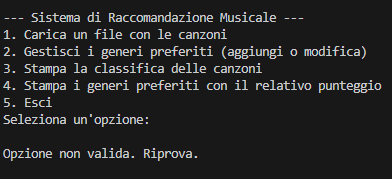
\includegraphics[width=0.5\textwidth]{htest1}
\end{center}
\begin{center}
    \textbf{Test 2}
    \par
    \vspace{0.5cm}
    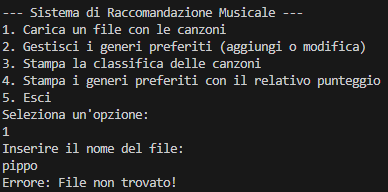
\includegraphics[width=0.5\textwidth]{htest2}
\end{center}
\begin{center}
    \textbf{Test 3}
    \par
    \vspace{0.5cm}
    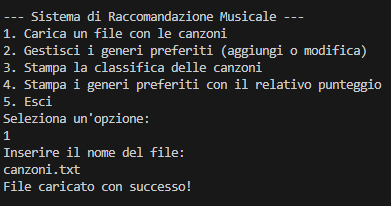
\includegraphics[width=0.5\textwidth]{htest3}
\end{center}

\newpage
\begin{center}
    \textbf{Test 4}
    \par
    \vspace{0.5cm}
    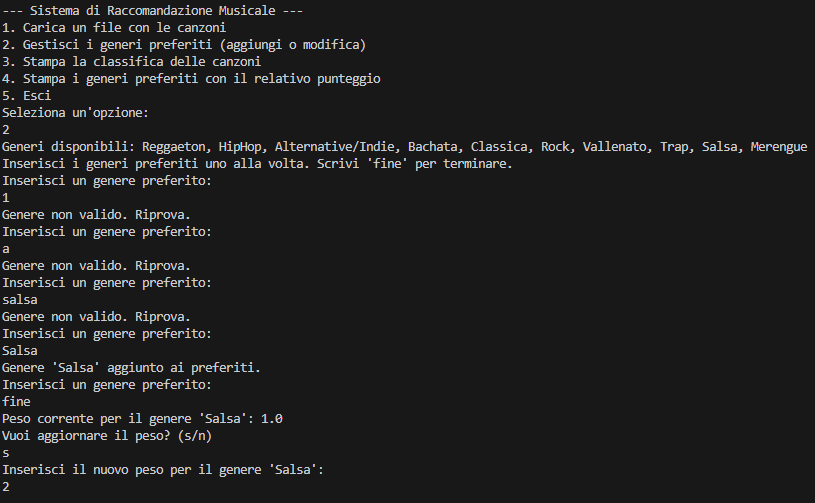
\includegraphics[width=0.5\textwidth]{htest4}
\end{center}
\begin{center}
    \textbf{Test 5}
    \par
    \vspace{0.5cm}
    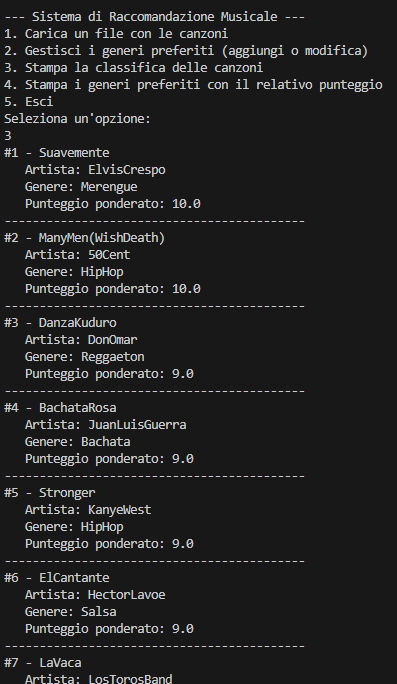
\includegraphics[width=0.5\textwidth]{htest5}
\end{center}

\newpage
\begin{center}
    \textbf{Test 6}
    \par
    \vspace{0.5cm}
    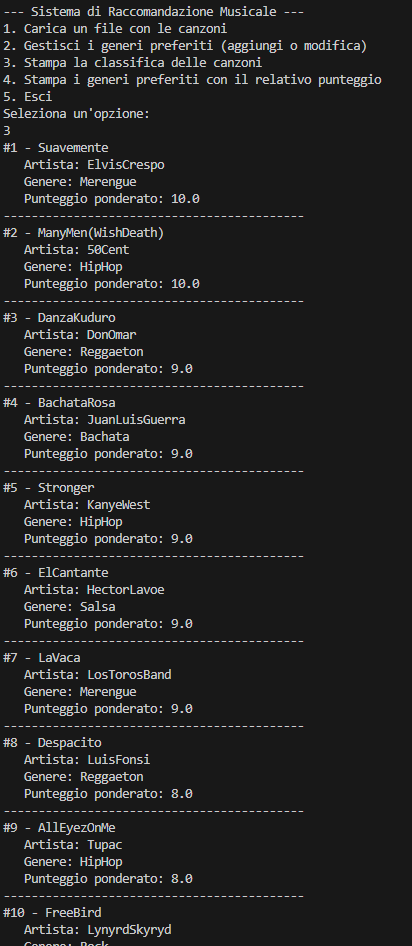
\includegraphics[width=0.5\textwidth]{htest6}
\end{center}
\begin{center}
    \textbf{Test 7}
    \par
    \vspace{0.5cm}
    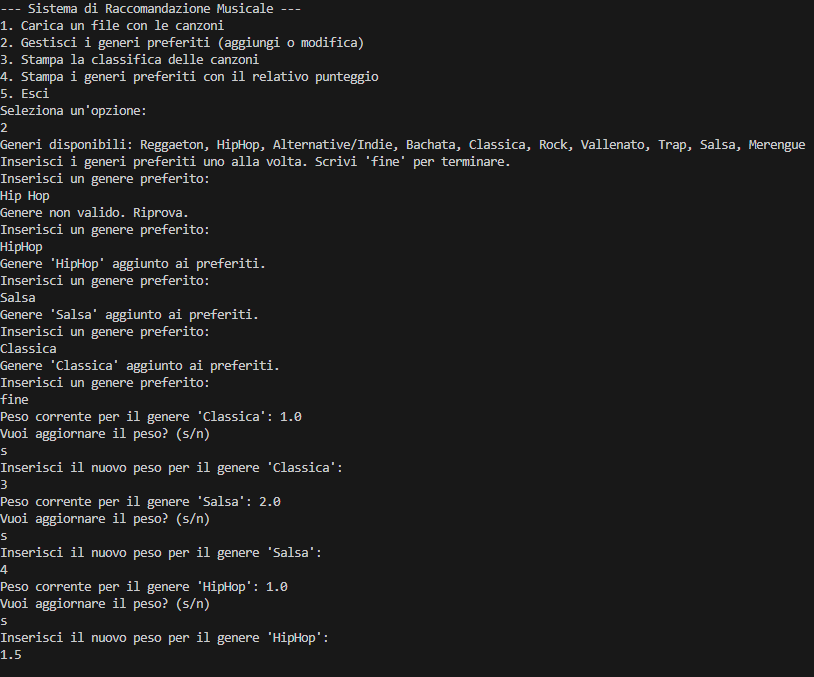
\includegraphics[width=0.5\textwidth]{htest7}
\end{center}
\begin{center}
    \textbf{Test 8}
    \par
    \vspace{0.5cm}
    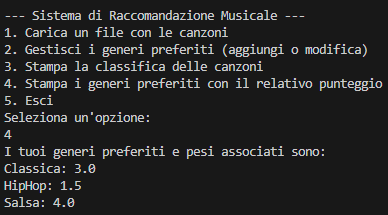
\includegraphics[width=0.5\textwidth]{htest8}
\end{center}

\newpage
\begin{center}
    \textbf{Test 9}
    \par
    \vspace{0.5cm}
    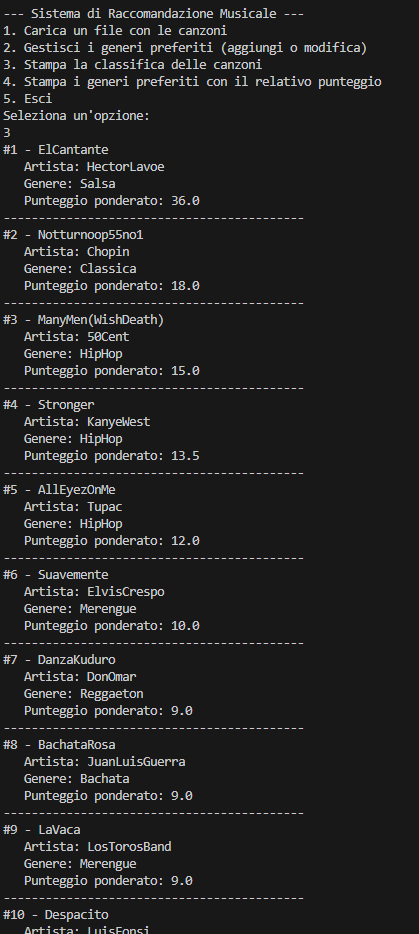
\includegraphics[width=0.5\textwidth]{htest9}
\end{center}
\begin{center}
    \textbf{Test 10}
    \par
    \vspace{0.5cm}
    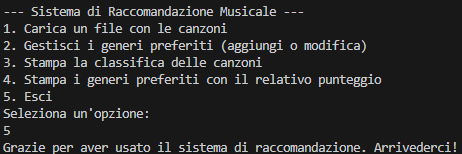
\includegraphics[width=0.5\textwidth]{htest10}
\end{center}
\vspace{1cm}

\newpage
\subsection{Testing del programma in Prolog}
\begin{center}
    \textbf{Test 1}
    \par
    \vspace{0.5cm}
    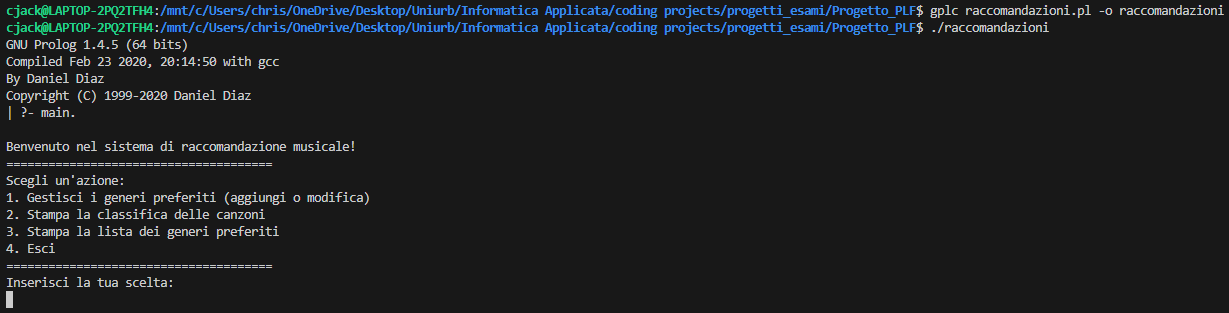
\includegraphics[width=0.5\textwidth]{ptest1}
\end{center}
\begin{center}
    \textbf{Test 2}
    \par
    \vspace{0.5cm}
    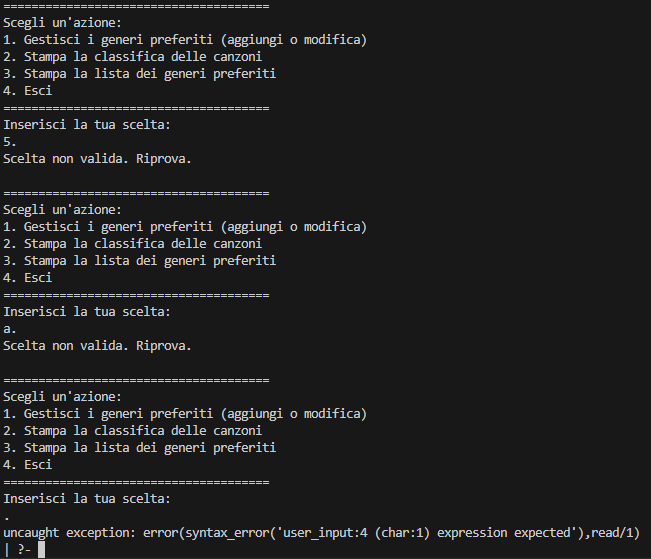
\includegraphics[width=0.5\textwidth]{ptest2}
\end{center}
\begin{center}
    \textbf{Test 3}
    \par
    \vspace{0.5cm}
    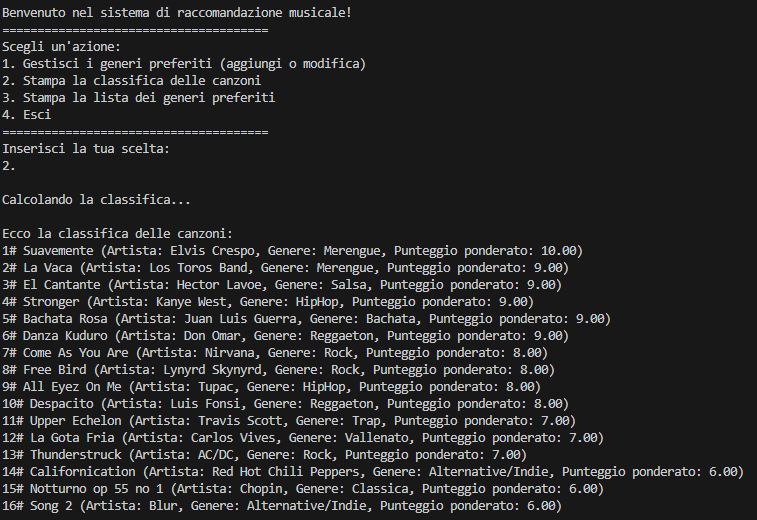
\includegraphics[width=0.5\textwidth]{ptest3}
\end{center}

\newpage
\begin{center}
    \textbf{Test 4}
    \par
    \vspace{0.5cm}
    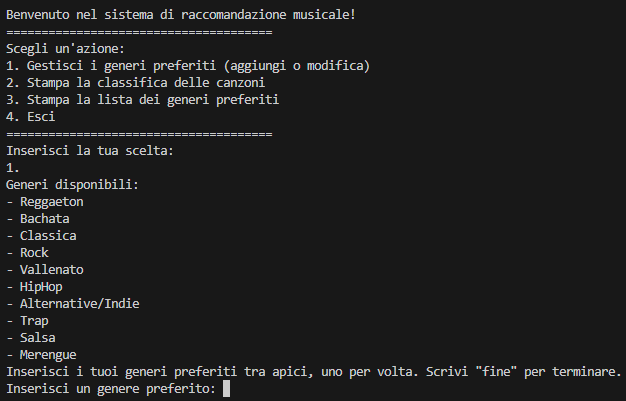
\includegraphics[width=0.5\textwidth]{ptest4}
\end{center}
\begin{center}
    \textbf{Test 5}
    \par
    \vspace{0.5cm}
    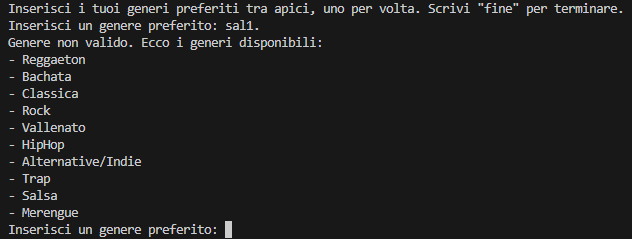
\includegraphics[width=0.5\textwidth]{ptest5}
\end{center}
\begin{center}
    \textbf{Test 6}
    \par
    \vspace{0.5cm}
    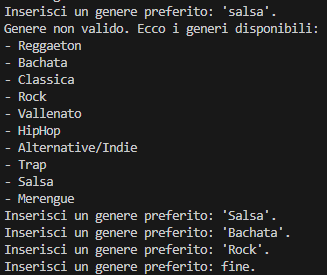
\includegraphics[width=0.5\textwidth]{ptest6}
\end{center}
\begin{center}
    \textbf{Test 7}
    \par
    \vspace{0.5cm}
    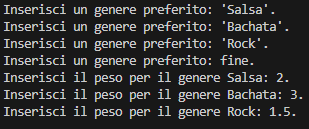
\includegraphics[width=0.5\textwidth]{ptest7}
\end{center}

\newpage
\begin{center}
    \textbf{Test 8}
    \par
    \vspace{0.5cm}
    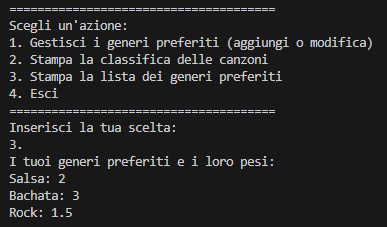
\includegraphics[width=0.5\textwidth]{ptest8}
\end{center}
\begin{center}
    \textbf{Test 9}
    \par
    \vspace{0.5cm}
    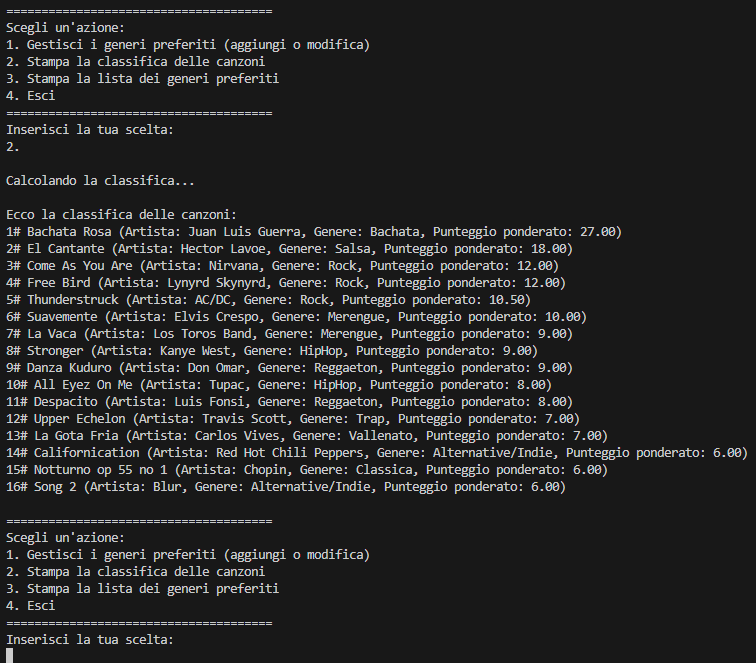
\includegraphics[width=0.5\textwidth]{ptest9}
\end{center}
\begin{center}
    \textbf{Test 10}
    \par
    \vspace{0.5cm}
    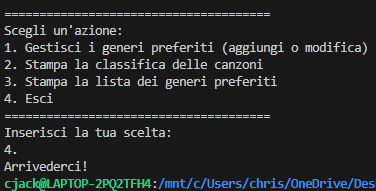
\includegraphics[width=0.5\textwidth]{ptest10}
\end{center}
\vspace{1cm}

\end{document}